\documentclass[professionalfonts, xcolor=dvipsnames, mathsans, 11pt, uncompressed]{beamer}

%\usepackage[czech]{babel}
%\usepackage[utf8]{inputenc}

\usepackage{tikz}
\usetikzlibrary{shapes,arrows,positioning,shadows,calc}
\usepackage{gnuplot-lua-tikz}

\usepackage{amsmath}
\usepackage{amsfonts}
\usepackage{amssymb}

\usepackage{cancel}
\usepackage{mathtools}
\usepackage{floatflt}
\usepackage{colortbl}
\usepackage{wasysym}
\usepackage{dcolumn}
\usepackage{units}

\usepackage{atbeginend}
\usepackage{graphicx}

\usepackage{ifthen}


\tikzstyle{mybox} = [draw=eqframecolor, fill=eqbgcolor, thick,
    rectangle, rounded corners, inner xsep=2pt, outer sep=0pt]
\tikzstyle{assumptions} = [draw=eqframecolor, fill=assumbgcolor, thick,
    rectangle, rounded corners, inner ysep=3ex, outer sep=0pt]
\tikzstyle{claims} = [draw=eqframecolor, fill=claimbgcolor, thick,
    rectangle, rounded corners, inner ysep=2ex, outer sep=1pt]
\tikzstyle{definebox} = [draw=eqframecolor, fill=defbgcolor, thick,
    rectangle, rounded corners, inner sep=1ex, outer sep=0pt, font=\small]        
\tikzstyle{fancytitle} =[fill=eqtitlebgcolor, text=eqtitlecolor, rounded corners, inner ysep=2pt]
\tikzstyle{term} = [inner sep=0pt,outer sep=0pt,anchor=base]
\tikzstyle{background grid}=[step=.1cm]

\newcommand{\eqnboxnamedl}[4][.8\textwidth]{%
	\begin{tikzpicture}[baseline]
		\node[mybox, inner ysep=2ex] (#2) {%
			\begin{minipage}[t]{#1}
				#4
			\end{minipage}
		};
	\node[fancytitle,inner sep=2pt, right=10pt] at (#2.north west) {#3};
	\end{tikzpicture}
}
\newcommand{\ddd}[4][]{%
	\node[definebox,#1] (#3) {%
		\begin{minipage}[t]{#2}
			{\color{structure}Define\\[-2ex]\hrule}
			#4
		\end{minipage}
	};
}
\newcommand{\eqnboxnamedc}[4][.8\textwidth]{%
	\begin{tikzpicture}[baseline]
		\node[mybox, inner ysep=2ex, inner xsep=2ex] (#2) {%
			\begin{minipage}{#1}\centering
				#4
			\end{minipage}
		};
	\node[fancytitle] (#2title) at (#2.north) {#3};
	\end{tikzpicture}
}
\newcommand{\eqnboxc}[2][.8\textwidth]{%
	\begin{tikzpicture}[baseline]
		\node[mybox] (box) {%
			\begin{minipage}[t]{#1}\centering
				#2
			\end{minipage}
		};
	\end{tikzpicture}
}

\newcommand{\bomega}{\ensuremath{\mathbf{\Omega}}}
\newcommand{\tinydot}{\mbox{\tiny{\textbullet}}}
\newcommand{\keff}{\ensuremath{k_{\mathrm{eff}}}}
\newcommand{\bx}{\ensuremath{\mathbf{x}}}
\newcommand{\bz}{\ensuremath{\mathbf{z}}}
\newcommand{\bn}{\ensuremath{\mathbf{n}}}
\renewcommand{\d}[1]{\ensuremath{\mathrm{d}#1\,}}
\newcommand{\dom}{\ensuremath{\Omega}}
\newcommand{\bnd}{\ensuremath{\partial\dom}}
\newcommand{\pd}[3][]{\ensuremath{\frac{\partial^{#1}#2}{\partial #3^{#1}}}}
\newcommand{\T}{\ensuremath{\mathcal{T}}}
\newcommand{\V}{\ensuremath{\mathcal{V}}}
\newcommand{\face}[1][]{\ensuremath{\Gamma\ifthenelse{\equal{#1}{}}{}{_{\mathrm{#1}}}}}
\newcommand{\on}[1]{\ensuremath{\ \mbox{on } \face[#1]}}
\newcommand{\abs}[1]{\ensuremath{\left\vert#1\right\vert}}
\newcommand{\Ra}{\ensuremath{\structure{\Rightarrow}}}

\newcommand{\ra}{\ensuremath{\!\rightarrow\!}}
\newcommand{\intv}[2][\d{\br}]{\ensuremath{\iiint_{\V_i}{#2}\,{#1}}}
\newcommand{\xint}[3]{\int_{#1}^{#2}{#3}\,\d{x}}

\newcommand{\Dnl}{\ensuremath{\widetilde{D}_{n\mid r}}}
\newcommand{\nod}[1][]{\ensuremath{^{\ifthenelse{\equal{#1}{}}{}{#1,}\mathrm{NOD}}}}
\newcommand{\cmfd}[1][]{\ensuremath{^{\ifthenelse{\equal{#1}{}}{}{#1,}\mathrm{CMFD}}}}

\newcommand{\fl}{\ensuremath{\phi}}
\newcommand{\afl}{\ensuremath{\psi}}
\newcommand{\flfl}{\ensuremath{\pmb{\phi}}}
\newcommand{\DD}{\ensuremath{\mathbf{D}_{\mathrm{kor}}}}
\newcommand{\MM}{\ensuremath{\mathbf{M}}}
\newcommand{\FF}{\ensuremath{\mathbf{F}}}
\newcommand{\QQ}{\ensuremath{\mathbf{Q}}}
\newcommand{\VV}{\ensuremath{\mathbb{V}}}
\newcommand{\EE}{\ensuremath{\mathbb{E}}}
\newcommand{\vv}{\ensuremath{\mathbf{v}}}


\newcommand{\rf}{\ensuremath{\mathrm{ref}}}

\renewcommand{\aa}[1]{\ensuremath{a^{#1}}}
\newcommand{\bb}[2]{\ensuremath{b^{#1#2}}}
\renewcommand{\ll}[1]{\ensuremath{l^{#1}}}
\renewcommand{\a}[3][]{\ensuremath{\ifthenelse{\equal{#1}{}}{a^{#2}(\fl^{#2},v^{#3})}{a^{#2}(\ltb{\fl^{#2}},\ltr{v^{#3}})}}}
\renewcommand{\b}[3][]{\ensuremath{\ifthenelse{\equal{#1}{}}{b^{#2#3}(\fl^{#3},v^{#2})}{b^{#2#3}(\ltb{\fl^{#3}},\ltr{v^{#2}})}}}
\renewcommand{\l}[1][]{\ensuremath{l^#1(v^{#1})}}
\newcommand{\A}{\ensuremath{\mathcal{A}}}
\renewcommand{\L}{\ensuremath{\ell}}
\newcommand{\enorm}[1]{\ensuremath{\lvert\lvert\lvert#1\rvert\rvert\rvert}}
\newcommand{\norm}[2][]{\ensuremath{\lvert\lvert#2\rvert\rvert_{#1}}}


\newcommand{\RR}[1][]{\ensuremath{\mathbb{R}^{#1}}}
\newcommand{\HH}[1][]{\ensuremath{H_{#1}^1(\dom)}}
\newcommand{\Linf}{\ensuremath{L^\infty(\dom)}}
\newcommand{\Ltwo}{\ensuremath{L^2(\dom)}}


\newcommand{\suma}{\sum_{\makebox[0pt]{${\scriptscriptstyle{g'\neq g}}$}}}
\newcommand{\io}[1]{\ensuremath{
	\structure{\stackrel{\mathrm{\tiny #1}}{\dashrightarrow}}}}
	
\newcommand{\dkg}[2][]{\bgroup\color#1{dkgreen}#2\egroup}
\newcommand{\dkb}[2][]{\bgroup\color#1{dkblue}#2\egroup}
\newcommand{\dkr}[2][]{\bgroup\color#1{dkred}#2\egroup}
\newcommand{\ltg}[2][]{\bgroup\color#1{green}#2\egroup}
\newcommand{\ltb}[2][]{\bgroup\color#1{blue}#2\egroup}
\newcommand{\ltr}[2][]{\bgroup\color#1{red}#2\egroup}
\newcommand{\gray}[2][]{\bgroup\color#1{black!60}#2\egroup}
\newcommand{\graysmall}[2][]{\bgroup\small\color#1{black!60}#2\egroup}


\newcommand{\mtx}[1]{\bigl[#1\bigr]}
\newcommand{\vct}[1]{\bigl\{#1\bigr\}}

%\newcolumntype{.}{D{.}{.}{-1}}

\newcommand{\invemph}[2][]{\color{white}#1{#2}\color#1{black}}
\newcommand{\tzterm}[3][black]{\tikz[baseline]\node[term,#1](#2){$#3$};}
\newcommand{\tztermrect}[3][.25ex]{%
	\tzterm[	fill=bg!65!blue,fill opacity=.5,text opacity=1,draw opacity=.5,
				color=structure.fg!85!bg,thin,draw,rectangle,rounded corners,inner sep=#1]
		{#2}{#3}
}
\newcommand{\tztermdisc}[2]{%
	\tikz[baseline]\node[term,fill=bg!85!blue,draw,circle,inner sep=0ex,yshift=-.5ex]
		(#1){$#2$};
}

\def\shorten#1#2{\bgroup%
\addtolength\abovedisplayshortskip{#1}%
\addtolength\abovedisplayskip{#1}%
\addtolength\belowdisplayshortskip{#2}%
\addtolength\belowdisplayskip{#2}%
}

\def\lengthen{\egroup}

%\color{black}

\setbeamercovered{invisible}

\mode<presentation>
{
	\usetheme{progressbar}
	%\usecolortheme{crane}
}
%\setlength{\textwidth}{11cm}
\title[Numerical methods for solving neutron diffusion problems] {
Comparison of Some Aspects of Nodal and \textit{hp}FEM Methods for Nuclear Reactor Simulation}

\author{\parbox[t]{4cm}{\hfill Milan Hanu{\v s}\hfill\ \\\hbox{} \hfill{\tiny Dept. of Mathematics, WBU Pilsen}\hfill\hbox{}\\[.6em]}}

\date{SIAM Conference on Computational Science and Engineering, Reno, Nevada. March $2^{\mathrm{nd}}$ 2011 }

\tikzstyle{every picture}+=[remember picture]

\AtBeginSection[]{%
	\addtocounter{framenumber}{-1}
  	\begin{frame}[t]
   	\frametitle{Overview}
   	\tableofcontents[currentsection]
	\end{frame}
}

\begin{document}


\definecolor{dkblue}{named}{blue}
\definecolor{dkgreen}{rgb}{0,0.4,0}
\definecolor{dkred}{rgb}{0.4,0,0}
\definecolor{dkgrey}{rgb}{0.4,0.4,0.4}
\definecolor{ltgrey}{rgb}{0.6,0.6,0.6}

\colorlet{shadow}{bg!92!blue}
\colorlet{rulecolor}{brown!50!yellow!15!black}
\colorlet{eqbgcolor}{brown!15!yellow!15!white}
\colorlet{assumbgcolor}{red!70!yellow!15!white}
\colorlet{claimbgcolor}{green!70!yellow!15!white}
\colorlet{defbgcolor}{blue!70!yellow!15!white}
\colorlet{eqtitlecolor}{orange!30}
\colorlet{eqtitlebgcolor}{structure}
\colorlet{eqframecolor}{structure}
\colorlet{bndcolor}{white!35!black}

\everymath{\displaystyle}


%===================================== TITLE ===================================
\progressbaroptions{frametitle=picture-section,titlepage=picture,imagename=images/unilogo}



\begin{frame}[label=s0]
	\titlepage
\end{frame}



%================================= MAIN CONTENT ===================================
\progressbaroptions{headline=sections,frametitle=normal}




\begin{frame}[label=s1]
	\frametitle{Overview}
	\tableofcontents
\end{frame}

\section{Mathematical-physical model}

\begin{frame}
	\frametitle{Nuclear reactor simulation }
	% TODO: provazani
	\begin{itemize}
		\item \alt<1-4>{Neutronics}{\emph{Neutronics}}
			\begin{itemize}
				\item Steady state problems (criticality, neutron flux field calculations)
				\item Transient problems (accident analyses)
				\item Inverse problems (neutron tomography)
			\end{itemize}\pause
		\item Coolant/moderator thermohydraulics
		\item Long term simulation
			\begin{itemize}
				\item fuel depletion, change of operating conditions, ...\\[1.5em]
			\end{itemize}		
	\end{itemize}
	\hfill\color{dkred}{\large fully coupled}\hfill\hbox{}
\end{frame}

\begin{frame}[t]
	\frametitle{Governing equations} 
	\begin{tikzpicture}[baseline,overlay]
		\node[mybox, below left=2cm and .05cm of current page.north, anchor=north, inner ysep=2ex, inner xsep=2ex] (treq) {%
			\begin{overlayarea}{\textwidth}{1.8cm}
				{
					\centering
					\only<1>{$\frac{1}{v}\pd{\afl}{t} + L\afl = (H+F)\afl + Q$\\[.3em]}
					\only<2>{$\frac{1}{v}\pd{\fl}{t}  + L\fl = (H+F)\fl + Q$\\[.3em]}
					\only<3>{$\frac{1}{v^g}\pd{\fl^g}{t} + L^{gg}\fl^g = \bigl(H^{gg'} + F^{gg'}\bigr)\fl^{g'} + Q^g, \quad g = 1,\ldots,G$\\[.3em]}
					\only<4>{\vspace*{.5ex}$L^{gg}\fl^g = \bigl(H^{gg'} + F^{gg'}\bigr)\fl^{g'} + Q^g, \quad g = 1,2,\ldots,G$\\[.3em]}
					\only<5>{\vspace*{.5ex}$L^{gg}\fl^g = \bigl(H^{gg'} + \lambda^{-1}F^{gg'}\bigr)\fl^{g'}, \quad g = 1,\ldots,G$\\[.3em]}
				}
				\color{white!35!black}\hrulefill\\
				\small\color{bndcolor}
				+ \only<1-3>{initial, }\only<5>{homogeneous }boundary conditions\\
				\only<1-3>{+ PDEs describing fission product kinetics}
			\end{overlayarea}
		};
		\node[fancytitle] (treqtitle) at (treq.north) {
			\only<1>{Linear Boltzmann transport equation}
			\only<2>{Diffusion approximation of neutron transport}
			\only<3>{Multigroup approximation}
			\only<4>{Steady state -- explicit sources (volumetric, boundary)}
			\only<5>{Steady state -- only implicit sources (fission)}
		};
	\end{tikzpicture}
	
	\begin{tikzpicture}[overlay]
	\node[below=.01cm of treq.south] {
		\begin{columns}[t]
		\begin{column}{.45\linewidth}
		\begin{itemize}
			\item\color{black} $L$ ... \alt<1>{transport}{diffusion} operator\\\graysmall{
			\alt<1-2>{(\alt<1>{1st}{2nd} order differential in $\bx$)}{(diagonal $G\!\times\!G$ matrix)}}
			\item\color{black} $H$ ... scattering operator\\\graysmall{ (\alt<1-2>{integral in $E$\only<1>{,$\bomega$}}{full $G\times G$ matrix})}
			\item\color{black} $F$ ... fission operator\\\graysmall{ (\alt<1-2>{integral in $E$\only<1>{,$\bomega$}}{full $G\times G$ matrix})}
			\item<1-4>\color{black} $Q$ ... explicit source \only<3->{\\\graysmall{($G\times1$ vector)}}
		\end{itemize}
		\end{column}
		\begin{column}{.55\linewidth}
		\begin{itemize}
			\item \temporal<2>{$\afl(\bz)$ \ldots angular neutron flux}{$\fl(\bz)$ ... isotropic neutron flux}{$\fl(\bx)$ ... isotropic neutron flux \only<3->{\graysmall{($G\times1$ vector)}}}
			\only<1-2>{
				\item $\bz = (\bx,E\only<1>{,\bomega})$\\
					$\hphantom{\bz = }$\graysmall{(space, energy\only<1>{, direction})}
				\item $v = v(E)$ ... neutron speed
			}
			\only<3>{
				\item $v^g$ ... avg. speed of neutrons\\ 
					$\hphantom{v^g}$\hphantom{ ...} in group $g$
			}				
			\item<3->\color{black} $g,g'$ ... energy groups
			\item<5> $\lambda_{\mathrm{max}}$ ... \emph{critical} eigenvalue\\$\hphantom{\lambda_{\mathrm{max}}\ldots\,}$(denote $\keff$)\\
			$\phi_{\mathrm{max}}$ ... \emph{fundamental} neut. flux
		\end{itemize}
		\end{column}
		\end{columns}
	};
	\end{tikzpicture}
	% TODO: eventuelně zmínit Batemanovy rovnice	
\end{frame}


\section{Finite volumes method}

\subsection{Standard FVM}
\begin{frame}[t]
	\frametitle{Finite volume method} 
	\only<1-6>{
		\eqnboxnamedc[.9\textwidth]{eqns}
		{
			\only<1>{\small Multigroup diffusion approximation, fixed source}
			\only<2>{\small Multigroup diffusion approximation, $g=1,\!\ldots\!,G$, fixed source}
			\only<3>{\small Integration over $\V_n$ (reactor core: $\Omega = \cup_n \V_n$), divergence thm.}
			\only<4->{\small Discrete formulation}
			\only<5->{\small Discrete formulation, \textit{"albedo"} B.C.}
		}
		{
		\begin{overlayarea}{\linewidth}{1.8cm}
			\centering
			\only<1>{$\vphantom{\suma}\mathbb{L}\Phi = (\mathbb{H}+\mathbb{F})\Phi + \mathbb{Q}$}
			\only<2>{
			$-\nabla\cdot\tzterm[dkgreen]{D}{D^g}\nabla\fl^g+\tzterm[dkgreen]{Sr}{\Sigma_r^g}\fl^g = \suma\tzterm[dkgreen]{Sgg}{\Sigma_s^{g\leftarrow g'}}\fl^{g'}
				 + \tzterm[dkgreen]{chi}{\chi^g}\!\sum_{g'}\tzterm[dkgreen]{nSf}{\nu\Sigma_f^{g'}}\fl^{g'} + Q^g$
			}
			\only<3>{
				$\sum_{r} j^g_{n\mid r}+\tzterm[dkgreen]{Sr}{\Sigma_{rn}^g}\fl_n^g = \suma\tzterm[dkgreen]{Sgg}{\Sigma_{sn}^{g\leftarrow g'}}\fl_n^{g'} 
				+	\chi^g\!\sum_{g'}\tzterm[dkgreen]{nSf}{\nu\Sigma_{fn}^{g'}}\fl_n^{g'} + Q_n^g$
			}
			\only<4>{
				$\sum_{r} j^g_{n\mid r}+\Sigma_{rn}^g\fl_n^g\ = \suma{\Sigma_{sn}^{gg'}}\fl_n^{g'} 
				+	\chi^g\!\sum_{g'=1}\nu\Sigma_{fn}^{g'}\fl_n^{g'} + Q_n^g\quad \mbox{in } \dom$
			}
			\only<5>{
				$\sum_{r} j^g_{n\mid r}+\Sigma_{rn}^g\fl_n^g\ = \suma{\Sigma_{sn}^{gg'}}\fl_n^{g'} 
				+	\chi^g\!\sum_{g'=1}\nu\Sigma_{fn}^{g'}\fl_n^{g'} + Q_n^g\quad \mbox{in } \dom$\\[2ex]
				$\tzterm[dkgreen]{gamma}{\gamma^g}\fl_{n\mid}^{g} - j^g_{n\mid} = 0\quad \mbox{on } \bnd$
			}
			
			\only<6>{
				$\sum_{r} j^g_{n\mid r}+\Sigma_{rn}^g\fl_n^g\ - \suma{\Sigma_{sn}^{gg'}}\fl_n^{g'} 
				-	\chi^g\!\sum_{g'=1}\nu\Sigma_{fn}^{g'}\fl_n^{g'} = Q_n^g\quad \mbox{in } \dom$\\[2ex]
				$\gamma^g\fl_{n\mid}^{g} - j^g_{n\mid} = 0\quad \mbox{on } \bnd$
			}
		\end{overlayarea}
		}
	}
	\begin{tikzpicture}[overlay]
		\only<2-3>{
			\node[above=0.175cm of eqns.south, 
						fill=eqbgcolor, text=dkgreen, 
						draw, drop shadow={opacity=.5,fill=structure!50!black}] (desc) {
							\alt<2>{physical parameters}{homogenized parameters}
			};
			\foreach \tgt in {Sr, Sgg, nSf}
				\draw[->,dkgreen,opacity=.5,thick] (desc) -- (\tgt);			
			\only<2>{ 
				\draw[->,dkgreen,opacity=.5,thick] (desc) -- (chi);	
				\draw[->,dkgreen,opacity=.5,thick] (desc) -- (D);	
			}
		}
		\only<5>{
			\node[below right= .35cm and .4cm of eqns.south, 
						mybox, text=dkgreen, 
						draw] (desc) {
						\begin{minipage}{.43\textwidth}\small
							$=1$ for symmetry,\\
							$=0.5$ for vacuum b.c.\\
							other typical bc: $\fl_{n\mid}=0$,\\
							\hphantom{other typical bc: ~}$j_{n\mid} = -J_0$ 
						\end{minipage}
			};
			\draw[->,dkgreen,opacity=.5,thick] (desc) -- (gamma);	
		}
	\end{tikzpicture}
	
	\only<2,3,4,6>{ 
		\begin{tikzpicture}[overlay]
			
			\only<2>{
				\node at (current page.south) [anchor=south,yshift=.55cm,xshift=-.55cm] {
					\definecolor{uququq}{rgb}{0.25,0.25,0.25}
\definecolor{wwqqff}{rgb}{0.0,0.7,0.4}
\definecolor{zzttqq}{rgb}{0.6,0.2,0}
\definecolor{qqwwff}{rgb}{0.8,0.9,1}
\definecolor{ttfftt}{rgb}{1,0.6,0.2}
\definecolor{qqttzz}{rgb}{0,0.4,0.6}
\definecolor{ffttww}{rgb}{0.8,0.2,0.4}
\definecolor{gggggg}{rgb}{0.8,0.7,1}
\definecolor{ffffff}{rgb}{0.5,0.8,0.9}
\begin{tikzpicture}[line cap=round,line join=round,>=triangle 45,x=0.65cm,y=0.65cm]
\clip(0,0) rectangle (7,7);

%1,1
\coordinate (A) at (0,2);
\coordinate (B) at (0,1);
\coordinate (C) at (0.87,0.5);
\coordinate (D) at (1.73,1);
\coordinate (E) at (1.73,2);
\coordinate (F) at (0.87,2.5);
\coordinate (origin) at (intersection of A--D and B--E);
% Draw the filled hex
\draw[top color=ffttww, bottom color=gggggg, shading angle=45] (A) -- (B) -- (C) -- (D) -- (E) -- (F) -- cycle;						

\draw[top color=qqttzz, shading angle=45 , bottom color=ffffff] (1.73,2) -- (1.73,1) -- (2.6,0.5) -- (3.46,1) -- (3.46,2) -- (2.6,2.5) -- cycle;				%2,1
\draw[bottom color=ttfftt, shading angle=-45 , top color=ffffff] (3.46,2) -- (3.46,1) -- (4.33,0.5) -- (5.2,1) -- (5.2,2) -- (4.33,2.5) -- cycle;				%3,1
\draw[top color=qqwwff, shading angle=45 , bottom color=ffffff] (2.6,3.5) -- (2.6,2.5) -- (3.46,2) -- (4.33,2.5) -- (4.33,3.5) -- (3.46,4) -- cycle;		%3,2
\draw[bottom color=qqttzz, shading angle=-45 , top color=gggggg] (0.87,3.5) -- (0.87,2.5) -- (1.73,2) -- (2.6,2.5) -- (2.6,3.5) -- (1.73,4) -- cycle;		%2,2
\draw[top color=zzttqq, shading angle=45 , bottom color=gggggg] (4.33,3.5) -- (4.33,2.5) -- (5.2,2) -- (6.06,2.5) -- (6.06,3.5) -- (5.2,4) -- cycle;  	%4,2
\draw[bottom color=zzttqq, shading angle=-45 , top color=gggggg] (3.46,5) -- (3.46,4) -- (4.33,3.5) -- (5.2,4) -- (5.2,5) -- (4.33,5.5) -- cycle; 			%4,3
\draw[top color=ttfftt, shading angle=45 , bottom color=ffffff] (1.73,5) -- (1.73,4) -- (2.6,3.5) -- (3.46,4) -- (3.46,5) -- (2.6,5.5) -- cycle;				%3,3
\draw[bottom color=wwqqff, shading angle=-45 , top color=ffffff] (5.2,2) -- (5.2,1) -- (6.06,0.5) -- (6.93,1) -- (6.93,2) -- (6.06,2.5) -- cycle;				%4,1
\draw[top color=wwqqff, shading angle=45 , bottom color=ffffff] (2.6,6.5) -- (2.6,5.5) -- (3.46,5) -- (4.33,5.5) -- (4.33,6.5) -- (3.46,7) -- cycle;		%4,4
\draw [color=ffttww] (0,2)-- (0,1);
\draw [color=ffttww] (0,1)-- (0.87,0.5);
\draw [color=ffttww] (0.87,0.5)-- (1.73,1);
\draw [color=ffttww] (1.73,1)-- (1.73,2);
\draw [color=ffttww] (1.73,2)-- (0.87,2.5);
\draw [color=ffttww] (0.87,2.5)-- (0,2);
\draw [color=qqttzz] (1.73,2)-- (1.73,1);
\draw [color=qqttzz] (1.73,1)-- (2.6,0.5);
\draw [color=qqttzz] (2.6,0.5)-- (3.46,1);
\draw [color=qqttzz] (3.46,1)-- (3.46,2);
\draw [color=qqttzz] (3.46,2)-- (2.6,2.5);
\draw [color=qqttzz] (2.6,2.5)-- (1.73,2);
\draw [color=ttfftt] (3.46,2)-- (3.46,1);
\draw [color=ttfftt] (3.46,1)-- (4.33,0.5);
\draw [color=ttfftt] (4.33,0.5)-- (5.2,1);
\draw [color=ttfftt] (5.2,1)-- (5.2,2);
\draw [color=ttfftt] (5.2,2)-- (4.33,2.5);
\draw [color=ttfftt] (4.33,2.5)-- (3.46,2);
\draw [color=qqwwff] (2.6,3.5)-- (2.6,2.5);
\draw [color=qqwwff] (2.6,2.5)-- (3.46,2);
\draw [color=qqwwff] (3.46,2)-- (4.33,2.5);
\draw [color=qqwwff] (4.33,2.5)-- (4.33,3.5);
\draw [color=qqwwff] (4.33,3.5)-- (3.46,4);
\draw [color=qqwwff] (3.46,4)-- (2.6,3.5);
\draw [color=qqttzz] (0.87,3.5)-- (0.87,2.5);
\draw [color=qqttzz] (0.87,2.5)-- (1.73,2);
\draw [color=qqttzz] (1.73,2)-- (2.6,2.5);
\draw [color=qqttzz] (2.6,2.5)-- (2.6,3.5);
\draw [color=qqttzz] (2.6,3.5)-- (1.73,4);
\draw [color=qqttzz] (1.73,4)-- (0.87,3.5);
\draw [color=zzttqq] (4.33,3.5)-- (4.33,2.5);
\draw [color=zzttqq] (4.33,2.5)-- (5.2,2);
\draw [color=zzttqq] (5.2,2)-- (6.06,2.5);
\draw [color=zzttqq] (6.06,2.5)-- (6.06,3.5);
\draw [color=zzttqq] (6.06,3.5)-- (5.2,4);
\draw [color=zzttqq] (5.2,4)-- (4.33,3.5);
\draw [color=zzttqq] (3.46,5)-- (3.46,4);
\draw [color=zzttqq] (3.46,4)-- (4.33,3.5);
\draw [color=zzttqq] (4.33,3.5)-- (5.2,4);
\draw [color=zzttqq] (5.2,4)-- (5.2,5);
\draw [color=zzttqq] (5.2,5)-- (4.33,5.5);
\draw [color=zzttqq] (4.33,5.5)-- (3.46,5);
\draw [color=ttfftt] (1.73,5)-- (1.73,4);
\draw [color=ttfftt] (1.73,4)-- (2.6,3.5);
\draw [color=ttfftt] (2.6,3.5)-- (3.46,4);
\draw [color=ttfftt] (3.46,4)-- (3.46,5);
\draw [color=ttfftt] (3.46,5)-- (2.6,5.5);
\draw [color=ttfftt] (2.6,5.5)-- (1.73,5);
\draw [color=wwqqff] (5.2,2)-- (5.2,1);
\draw [color=wwqqff] (5.2,1)-- (6.06,0.5);
\draw [color=wwqqff] (6.06,0.5)-- (6.93,1);
\draw [color=wwqqff] (6.93,1)-- (6.93,2);
\draw [color=wwqqff] (6.93,2)-- (6.06,2.5);
\draw [color=wwqqff] (6.06,2.5)-- (5.2,2);
\draw [color=wwqqff] (2.6,6.5)-- (2.6,5.5);
\draw [color=wwqqff] (2.6,5.5)-- (3.46,5);
\draw [color=wwqqff] (3.46,5)-- (4.33,5.5);
\draw [color=wwqqff] (4.33,5.5)-- (4.33,6.5);
\draw [color=wwqqff] (4.33,6.5)-- (3.46,7);
\draw [color=wwqqff] (3.46,7)-- (2.6,6.5);
\end{tikzpicture}

				};
			}
			\only<3>{
				\node at (current page.south) [anchor=south,yshift=.75cm] {
					\includegraphics[scale=.45]{images/core.pdf}
				};
			}
			\only<4,6>{
				\node at (current page.east) [anchor=east,yshift=-0.9cm,xshift=-2.1cm] {\definecolor{uququq}{rgb}{0.25,0.25,0.25}
\definecolor{zzttqq}{rgb}{0.6,0.2,0}
\definecolor{gattac}{rgb}{0,0.2,0.6}
\definecolor{qqqqff}{rgb}{0,0,0}
\begin{tikzpicture}[line cap=round,line join=round,>=triangle 45,x=2cm,y=2cm]
\clip (0.9,0.5) rectangle (2.6,2.1);
\fill[color=zzttqq,fill=zzttqq,fill opacity=0.25] (1,1) -- (2,1) -- (1.5,1.87) -- cycle;
\fill[color=gattac,fill=gattac,fill opacity=0.25] (2.5,1.87) -- (2,1) -- (1.5,1.87) -- cycle;
\draw [color=zzttqq] (1,1)-- (2,1);
\draw [color=zzttqq] (2,1)-- (1.5,1.87);
\draw [color=zzttqq] (1.5,1.87)-- (1,1);
\draw [color=gattac] (2.5,1.87)-- (2,1);
\draw [color=gattac] (2,1)-- (1.5,1.87);
\draw [color=gattac] (1.5,1.87)-- (2.5,1.87);
\draw [<->] (1.85,0.68) -- (2.35,0.97);
\draw [dash pattern=on 1pt off 1pt] (1.5,1.29)-- (1.85,0.68);
\draw [dash pattern=on 1pt off 1pt] (2,1.58)-- (2.35,0.97);
\draw (2.05,0.83) node[anchor=north west] {\small$h$};
\draw (1.73,1.68) node[anchor=center,rotate=-60] {$n\mid r$};
\draw (1.24,1.16) node[anchor=center] {$\V_n$};
\draw (2.22,1.73) node[anchor=center] {$\V_r$};
\fill [color=uququq] (1.5,1.29) circle (1.5pt);
\fill [color=uququq] (2,1.58) circle (1.5pt);
\end{tikzpicture}
};
			}
		\end{tikzpicture}	
	}
	\only<4-6>{
		\begin{tikzpicture}[overlay]
			\node[mybox, inner sep = 1ex, below=2ex of eqns.south west, anchor=north west] (box1) {	
				\begin{minipage}[t]{.4\textwidth}\centering
					\small
					$\fl_n = \frac{1}{\abs{\V_n}} \int_{\V_n} \fl(\bx)\d{\bx}$\\[2ex]
					%\only<4>{
					%	\tikz[baseline]\node [anchor=text,rounded corners,draw=dkgreen] (FZ) {
					%		$j_{n\mid r} = -\bn\cdot D_{n\mid r} \nabla \fl_{n\mid r}$
					%	};
					%}
					\only<4-6>{
						$j_{n\mid r} = -\bn\cdot D_{n\mid r} \nabla \fl_{n\mid r}$
					}
					%\only<6>{
					%	$j_{n\mid r} \approx -\Dnl (\fl_r - \fl_n)$\\[2ex]$\Dnl = \frac{2 D_n D_r}{h(D_n + D_r)}$
					%}
				\end{minipage}
			};
	        \only<6>{
                \node[mybox, inner ysep=2ex, inner xsep=2ex, below=6ex of box1.south west, anchor=north west] (box2) {%
			            \begin{minipage}[t]{.9\textwidth}\centering
				            $\MM\flfl = \QQ$
			            \end{minipage}
		            };
	            \node[fancytitle] (box2title) at (box2.north) {System of linear algebraic equations};
            }
		\end{tikzpicture}
	}
%	\begin{tikzpicture}[overlay]
%		\only<4>{
%			\node[below=.5cm of FZ.south, 
%						fill=eqbgcolor, text=dkgreen, 
%						draw, drop shadow={opacity=.5,fill=structure!50!black}] (desc) {
%							Fick's law
%			};
%			\draw[->,dkgreen,opacity=.5,thick] (desc) -- (FZ);
%		}
%	\end{tikzpicture}
\end{frame}

\begin{frame}
	\frametitle{Finite volume method -- eigenvalue problem} 
	\begin{center}
		\eqnboxnamedc[.7\textwidth]{eqns}
		{
			Reactor criticality calculation
		}
		{
			$\MM\flfl = \frac{1}{\keff}\FF\flfl$
		}\\[2em]
		\eqnboxnamedc[.7\textwidth]{pi}{\textit{Source iteration}}{
			\shorten{-.3cm}{-.5cm}
			\begin{align*}
				 \MM\flfl^{(n)} &= \color{dkblue}\frac{1}{\keff^{(n-1)}}\FF\flfl^{(n-1)} \quad \mbox{ \color{dkblue}(fixed source $\mathbf{S}_f^{(n-1)}$) }\\
				 \keff^{(n)} &= \keff^{(n-1)} \frac{\norm{\FF\flfl^{(n)}}}{\norm{\FF\flfl^{(n-1)}}}
			\end{align*}
			\lengthen
		}
	\end{center}		
\end{frame}


\subsection{Nodal method}
\begin{frame}[t]
	\frametitle{Nodal method} 
	\eqnboxnamedc[.9\textwidth]{eqns}	{\small Nodal equation for each node $\V_n$}
	{
		\begin{overlayarea}{\linewidth}{1.1cm}
			\centering
			$\vphantom{\sum_a^b}
			\sum_{r} \hat{j}_{n\mid r}^g+{\Sigma_{rn}^g}\hat\fl_n^g - \suma{\Sigma_{sn}^{gg'}}\hat\fl_n^{g'} - \chi^g\!\sum_{g'=1}\nu\Sigma_{fn}^{g'}\hat\fl_n^{g'}
			=	Q_n^g$
		\end{overlayarea}
	}
	
	\begin{tikzpicture}[overlay]
		\node[mybox, inner sep = 1ex, below=2ex of eqns.south west, anchor=north west] (box1) {
			\begin{minipage}[c]{.45\textwidth}
				$\hat\fl_n(x,y) \approx \fl_n + \sum_{i=1}^{K}c_i f_i(x,y)$ \\[2ex]
				$\hat{j}_{n\mid r} \approx -\bn\cdot\Dnl\nabla \left.\hat\fl_n(x,y)\right\vert_{n\mid r}$
			\end{minipage}
		};
		\node[fancytitle,inner sep=2pt,xshift=.5em,anchor=west] at (box1.north west) {\footnotesize Nodal expansion};				
		\node [inner sep=0pt, below right=2.5ex and 1ex of eqns.south east, anchor=north east] (box2) {
			\only<1-2>{
				%\documentclass[10pt]{article}
%\usepackage{pgf,tikz}
%\usetikzlibrary{arrows}
%\pagestyle{empty}
%\newcommand{\V}{\ensuremath{\mathcal{V}}}
%\begin{document}

\definecolor{uququq}{rgb}{0,0,0}
\definecolor{ffttww}{rgb}{0.6,0.2,0}
\definecolor{qqttzz}{rgb}{0,0.2,0.6}
\begin{tikzpicture}[line cap=round,line join=round,>=triangle 45,x=0.85cm,y=0.85cm]
\clip(-.1,.5) rectangle (4,4);
%\draw[step=1cm,color=blue!30] (0,0) grid (10,10);
\fill[color=ffttww,fill=ffttww,fill opacity=.25] (0,2) -- (0,1) -- (0.87,0.5) -- (1.73,1) -- (1.73,2) -- (0.87,2.5) -- cycle;
\fill[color=qqttzz,fill=qqttzz,fill opacity=.25] (1.73,2) -- (1.73,1) -- (2.6,0.5) -- (3.46,1) -- (3.46,2) -- (2.6,2.5) -- cycle;
\fill[color=qqttzz,fill=qqttzz,fill opacity=.25] (0.87,3.5) -- (0.87,2.5) -- (1.73,2) -- (2.6,2.5) -- (2.6,3.5) -- (1.73,4) -- cycle;
\draw [color=ffttww] (0,2)-- (0,1);
\draw [color=ffttww] (0,1)-- (0.87,0.5);
\draw [color=ffttww] (0.87,0.5)-- (1.73,1);
\draw [color=ffttww] (1.73,1)-- (1.73,2);
\draw [color=ffttww] (1.73,2)-- (0.87,2.5);
\draw [color=ffttww] (0.87,2.5)-- (0,2);
\draw [color=qqttzz] (1.73,2)-- (1.73,1) node[midway,sloped,above,black]{\small$n\mid r_1$};
\draw [color=qqttzz] (1.73,1)-- (2.6,0.5);
\draw [color=qqttzz] (2.6,0.5)-- (3.46,1);
\draw [color=qqttzz] (3.46,1)-- (3.46,2);
\draw [color=qqttzz] (3.46,2)-- (2.6,2.5);
\draw [color=qqttzz] (2.6,2.5)-- (1.73,2);
\draw [color=qqttzz] (0.87,3.5)-- (0.87,2.5);
\draw [color=qqttzz] (0.87,2.5)-- (1.73,2) node[midway,sloped,above,black]{\small$n\mid r_2$};
\draw [color=qqttzz] (1.73,2)-- (2.6,2.5);
\draw [color=qqttzz] (2.6,2.5)-- (2.6,3.5);
\draw [color=qqttzz] (2.6,3.5)-- (1.73,4);
\draw [color=qqttzz] (1.73,4)-- (0.87,3.5);
\draw (0.83,1.5) node[anchor=center,black] {$\V_n$};
\draw (2.65,2) node[anchor=center,black] {$\V_{ r_1}$};
\draw (1.78,3.58) node[anchor=center,black] {$\V_{ r_2}$};
\draw [dash pattern=on 2pt off 2pt] (2.60,1.50)-- (3.90,2.25);
\draw [dash pattern=on 2pt off 2pt] (1.73,3.00)-- (3.03,3.75);
\draw (3.9,2.25) [<->] -- (3.03,3.75) node[midway,above,anchor=south west]{$h$};
\draw [color=gray] (0.43,2.25) [->] -- (-0.07,3.12);
\draw (0.33,2.75) node[anchor=center,gray] {$\mathbf{n}$};
\fill [color=uququq] (1.76,3.00) circle (1.0pt);
\fill [color=uququq] (2.60,1.50) circle (1.0pt);
\end{tikzpicture}

%\end{document}

			}
			\only<3->{
				\begin{minipage}[t]{.45\textwidth}
					\centering\emph{Conditions for $c_i$}\\[.5ex]\hrule
					\begin{itemize}
					 	\item corner-point balance,\\
					 	      system boundary conds.,\\
					 	      internodal continuity conds.\\
					 	\item weighted residual method
					\end{itemize}
				\end{minipage}
			}
		};
		\only<1-4>{
			\node[inner sep = 0pt, below=2.0ex of box1.south west, anchor=north west] (box3) {
				\begin{minipage}[t]{\textwidth}\small
					\begin{itemize}
							\item \alert<2>{suitable choice of $K$ and $\left\{f_i\right\}$} to allow coarser spatial discretization
									 			\uncover<2->{\\\Ra polynomial/semi-analytic/analytic nodal method}
							\item<4> relies on the \alert<4>{saturation assumption}:~
							$
							    \norm{\fl^* - \hat\fl} \leq \beta \norm{\fl^* - \fl},
							$~ where\\[.25em]
							$\fl^*$ repr. exact solution, $0 < \beta < 1$ and $\hat\fl|_{\V_n} = \hat\fl_n$ for each node $\V_n$
																 			
					\end{itemize}
				\end{minipage}
			};
		}
		\only<5>{
			\node[inner sep = 0pt, below=2.0ex of box1.south west, anchor=north west] (box3) {
				\begin{minipage}[t]{\textwidth}\small
					\begin{itemize}
						\item nodal methods based on transverse integration:
							\begin{itemize}\addtolength{\itemsep}{-.075\baselineskip}
								\item<5> simpler and more effective solution in separate coordinate directions
								\item<5> approximate coupling with other directions (\textit{"transverse leakage"})
								\item<5> \alert{information loss} $\Ra$ delicate reconstruction of the original solution
							\end{itemize}
					\end{itemize}
				\end{minipage}
			};
		}
	\end{tikzpicture}
\end{frame}	


\begin{frame}[t]
	\frametitle{Nodal method -- matrix formulation} 
	\centering
	\eqnboxnamedc[.9\textwidth]{eqns}
	{
		\only<1>{\small Nodal scheme (solve for each node $\V_n$)}
		\only<2->{\small FVM on a coarse mesh (a.k.a. CMFD)}
	}
	{
		\only<1>{
			\begin{overlayarea}{\linewidth}{1.1cm}
				\centering	
					$\vphantom{\sum_a^b}
					\sum_{r} \hat{j}_{n\mid r}^g+{\Sigma_{rn}^g}\hat\fl_n^g - \suma{\Sigma_{sn}^{gg'}}\hat\fl_n^{g'} - \chi^g\!\sum_{g'=1}\nu\Sigma_{fn}^{g'}\hat\fl_n^{g'}
					=	Q_n^g$
			\end{overlayarea}
		}
		\only<2->{
			\begin{overlayarea}{\linewidth}{.4cm}
%			\vspace*{.5em}
			\centering
			    $(\dkb{\MM} + \dkr{\DD})\flfl = \QQ$
			\end{overlayarea}
		}
	}
	
	\begin{tikzpicture}[overlay]
		\node[mybox, inner sep = 1ex, below=2ex of eqns.south, anchor=north] (box1) {
			\begin{minipage}[c]{.7\textwidth}
				\emph{NOD:} 
					$\hat{j}_{n\mid r} \approx -\bn\cdot\Dnl\nabla \!\!\left.\hat\fl_n(x,y)\right\vert_{n\mid r}$\\
				\only<3->{\hbox{}\hfill\dkr{$\Updownarrow$}\hfill\hbox{}\\}
				\only<2->{
					\emph{FVM:} $j_{n\mid r} \approx \dkb{-\Dnl}(\phi_r - \phi_n) + 
						\only<2>{
							\dkr{\widehat D_{n\mid r}}
						}
						\only<3->{	
							\tikz[baseline] \node [outer sep=8pt,inner sep=2pt, anchor=text,draw=dkred,thin,rounded corners] {$\dkr{\widehat D_{n\mid r}}$};
						}
						(\fl_n + \fl_r)$
				}
			\end{minipage}
		};		
		\node[inner sep = 0pt, below left=2.0ex and 1.5cm of box1.south west, anchor=north west] (box3) {
			\begin{minipage}[t]{\textwidth}\small
				\begin{itemize} 
					\only<1>{
					 \item \structure{NOD}al method: node by node, coupled by continuity of $\hat j_{n\mid r}$, $\hat \fl_{n\mid r}$
					 \item possible formulation as a single, banded matrix problem
					}
%					\item<2-> Combination with FVM possible%\vspace{-.2em}
%					\begin{itemize}
          \only<2->{
						\item FVM as an acceleration of NOD 
						\item NOD as a correction of coarse-mesh FVM discretization\only<2>{\\
										\structure{$\Ra$} nonlinear method coupled by factors $\dkr{\hat D_{n\mid r}}$:}
					}
%					\end{itemize}
				\end{itemize}
			\end{minipage}
		};

        \only<2->{
        \node[below=4pt of box3.south, anchor=north, inner ysep=0pt] (boxxxx) {%
            \begin{minipage}[t]{.7\textwidth}\centering
                $\dkr{\widehat D_{n\mid r}} = \frac{\hat{j}_{n\mid r} + \Dnl(\phi_r - \phi_n)}{\phi_n + \phi_r}$ 
            \end{minipage}
        };}
%        \only<3->{
%        \node[mybox, below=1.4em of box3.south, anchor=north, inner ysep=0pt] (boxx) {%
%            \begin{minipage}[t]{.7\textwidth}\centering
%                $$
%                \begin{aligned}
%                    \dkb{\MM}\flfl^{(n+\frac12)} = \QQ - \dkr{\DD}\flfl^{(n)}\\
%                    \dkr{\DD}\flfl^{(n+1)} = \QQ - \dkb{\MM}\flfl^{(n+\frac12)}
%                \end{aligned}
%                $$\\[.1em]
%            \end{minipage}
%        };
%        \node[fancytitle] (boxxt) at (boxx.north) {\small Iterative form};
%        }
        
	\end{tikzpicture}
		
	%TODO: vlastnosti matic
\end{frame}	

\begin{frame}[t]
	\frametitle{Nodal method -- pros and cons} 
	\vspace*{1cm}
	\begin{itemize}
		\item<1-> \dkg{Very fast, memory efficient, well-suited for parallelization}
		\item<1-> \dkg{Good for retrieving global information ($\keff$, average flux)\\[1em]}
		\item<2-> \dkr{Requires high-quality coarse-mesh data\\ (non-trivial homogenization/equivalence procedures)}	
		\item<2-> \dkr{For detailed flux distribution, most nodal methods require involved \textit{aposteriori} reconstruction}
		\item<2-> \dkr{Highly geometry-dependent}
		\item<2-> \dkr{Complicated theoretical analysis (order of accuracy, convergence)}
	\end{itemize}	
	\only<2->{
		\vspace{.15cm}\color{Black}\hrule width 5.1cm
		\begin{thebibliography}{\textwidth} 
			\beamertemplatearticlebibitems
			\bibitem[CMFD]{CMFD}
			\footnotesize{Deokjung Lee},
			\newblock \scriptsize{{C}onvergence {A}nalysis of the {C}oarse {M}esh {F}inite {D}ifference {M}ethod}
			\newblock \color{Black}Ph.D. Thesis, Purdue University, 2003      
		\end{thebibliography}		
	}
\end{frame}

\subsection{Practical realization}
\begin{frame}[t]
  \frametitle{HanKa}
  \begin{itemize}
  	\item \small Code for neutronics calculations of the VVER reactors
  \end{itemize}
  \pause
  \begin{tikzpicture}
			\node[mybox, inner ysep=1.2ex, inner xsep=0ex] (work) {%
				\begin{minipage}{1.03\textwidth}\centering
					\begin{itemize}
						\item \small\underline{R. Ku{\v z}el}, M. Brandner, M. Hanu{\v s}, M. Smitkov{\' a}, T. Berka$^{\dagger (2010)}$
						\item \small cooperation with Czech nuclear industry \structure{+} consultant V.G. Zimin$^{\scriptsize 1}$
					\end{itemize}
				\end{minipage}
			};
		\node[fancytitle] (worktitle) at (work.north) {\small People};
	\end{tikzpicture}
	\begin{tikzpicture}[overlay]
  	\node[font=\scriptsize, color=bg!92!fg, anchor=south west,yshift=.1cm] at (current page.south west) {$^1$ Moscow Engineering Physics Institute};
	\end{tikzpicture}\vspace{-.475cm}
  \pause
  \begin{tikzpicture}
			\node[mybox, inner ysep=1.2ex, inner xsep=0ex] (Model) {%
				\begin{minipage}{1.03\textwidth}\centering
					\small
					\begin{itemize}
            \item Multigroup diffusion approximation 
            \item Steady state (quasi-steady calculations for fuel optimization problems)
          \end{itemize}
				\end{minipage}
			};
		\node[fancytitle] (Modelt) at (Model.north) {\small Model};
	\end{tikzpicture}
  \pause
  \begin{tikzpicture}
			\node[mybox, inner ysep=1.2ex, inner xsep=0ex] (Method) {%
				\begin{minipage}{1.03\textwidth}\centering
					\small
					\begin{itemize}
            \item Nodal method (CMFD) based on conformal mapping (hex $\rightarrow$ rect)
            \item Fine-mesh method mainly for (de-)homogenization purposes
          \end{itemize}
				\end{minipage}
			};
		\node[fancytitle] (Methodt) at (Method.north) {\small Method};
	\end{tikzpicture}
  \pause
  \begin{tikzpicture}
			\node[mybox, inner ysep=1.2ex, inner xsep=0ex] (Implementation) {%
				\begin{minipage}{1.03\textwidth}\centering
					\small
          \begin{itemize}
            \item C++, parts of code generated by Mathematica, OpenMP
            \item 2D, layered 3D with approximate interlayer coupling
          \end{itemize}
				\end{minipage}
			};
		\node[fancytitle] (Implementationt) at (Implementation.north) {\small Implementation};
%		\node[anchor=east, left=2pt of Implementation.east]{
%		    \includegraphics[scale=.13]{images/HanKa/coreT.png}
%		};
	\end{tikzpicture}		
\end{frame}

\begin{frame}[c]
  \frametitle{HanKa -- V \& V}
%  \vspace*{-.25cm}
 
 \begin{itemize}
    \item Comparison on several standard criticality benchmarks for VVER-1000 and VVER-440 reactors
        \begin{itemize}
            \item[-] w.r.t. the solution independently computed with the same set of parameters by V. G. Zimin
            \item[-] w.r.t. the FV solution on a highly refined mesh
        \end{itemize}
  \end{itemize}      
  \vspace{3cm} \hrule width 5.1cm \vspace{-0.1cm}
	\begin{thebibliography}{\textwidth} 
	  \beamertemplatearticlebibitems
		\bibitem{ChaoShatilla95}
    {\footnotesize Y.~A.~Chao and Y.~A.~Shatilla}
    \newblock {\scriptsize Conformal Mapping and Hexagon. Nodal Methods II: Impl. in the ANC-H Code}. 
    \newblock {\scriptsize \color{black}Nucl. Sci. Eng., 121 (1995)}
	\end{thebibliography}
\end{frame}

\begin{frame}[t]
  \frametitle{HanKa -- V \& V}
  \vspace*{-.3cm}
  \centering\textcolor{structure.bg!95!blue}{ Assembly average power distribution comparisons }\\[-.3em]
  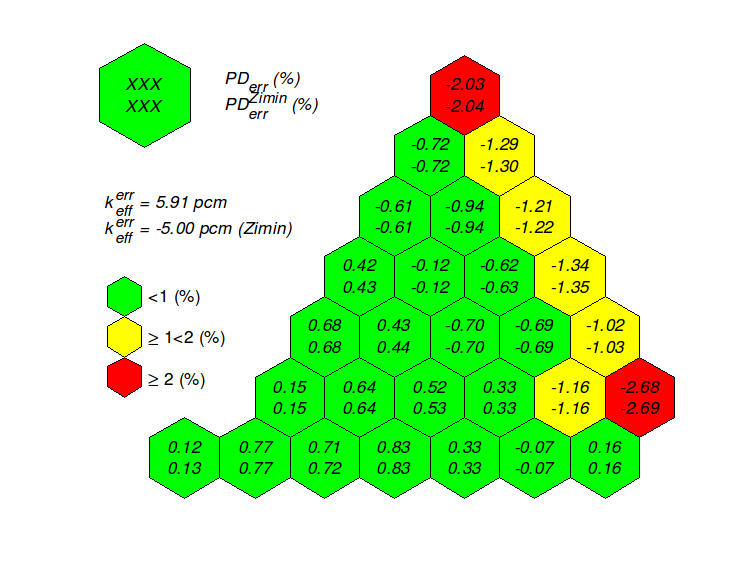
\includegraphics[scale=.5]{images/HanKa/HCZ1T.png}
  \vspace{-.7cm} \hrule width 5.1cm \vspace{-0.1cm}
	\begin{thebibliography}{\textwidth} 
	  \beamertemplatearticlebibitems
		\bibitem{ZiminBaturin02}
    {\scriptsize V.~G.~Zimin and D.~M.~Baturin}
    \newblock {\scriptsize Polynom. Nod. Meth. for Solving Neutron Dif. Eqns. in Hex-Z Geometry}. 
    \newblock {\scriptsize \color{white!80!black}Ann. Nucl. En. 29 (2002)}
	\end{thebibliography}
\end{frame}

\begin{frame}[t]
  \frametitle{HanKa -- V \& V}
  \vspace*{-.3cm}
  \centering\textcolor{structure.bg!95!blue}{ Assembly average power distribution comparisons}\\[-.3em]
  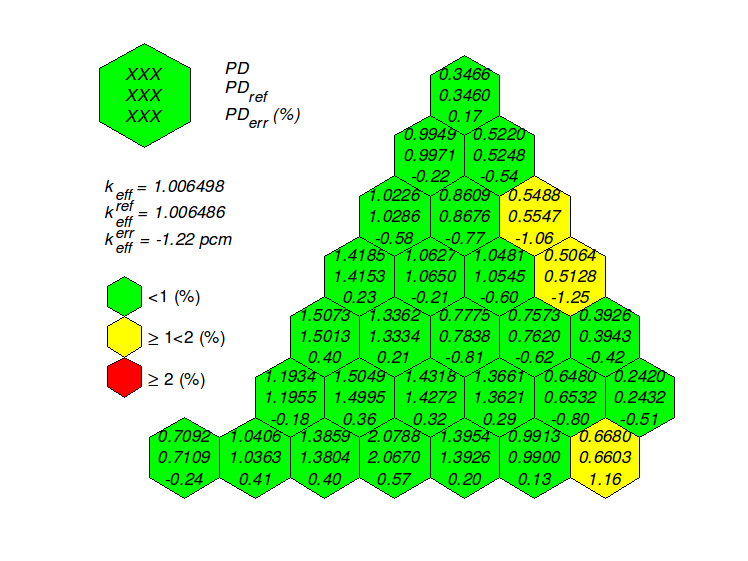
\includegraphics[scale=.5]{images/HanKa/HCZ2T.png}
  \vspace{-.85cm} 
  \begin{center} Modified treatment of boundary nodes \end{center}
\end{frame}


\section{Finite elements method}

\begin{frame}[c]
	\frametitle{Finite elements method} 
	\begin{tikzpicture}[overlay]
		\node[mybox, below left=1.6cm and .075cm of current page.north, anchor=north, inner ysep=2ex, inner xsep=2ex] (eqns) {%
			\begin{minipage}{\textwidth}\centering
				\only<1-5>{
						\begin{overlayarea}{\linewidth}{2.6cm}
						\centering
						\only<1-2>{\small
							\shorten{-1em}{-1em}
							\begin{align*}
								-\nabla\cdot D^g\nabla\fl^g+\Sigma_r^g\fl^g-\suma\Sigma_s^{gg'}\fl^{g'}
								 	- \chi^g\!\sum_{g'}\nu\Sigma_f^{g'}\fl^{g'} &= Q^g \quad \mbox{in } \dom\\
								 	\fl^g &= 0\quad \on{\fl}\\
								 	-\bn\cdot D^g\nabla \fl^g &= 0\quad \on{sym}\\ 
								 	 \bn\cdot D^g\nabla \fl^g + \gamma^g\fl^g &= 0\quad \on{\gamma}
							\end{align*}
							\lengthen
						}
						\only<3-4>{\small
							For $g=1,\ldots,G$ find $\fl^g\in V,$ such that $\forall v^g\in V$
							\begin{multline*}
								-\alert{\bigl(v^g,}\nabla\cdot D^g\nabla\fl^g\alert{\bigr)}+\alert{\bigl(v^g,}\Sigma_r^g\fl^g\alert{\bigr)}-\alert{\bigl(v^g,}\suma\Sigma_s^{gg'}\fl^{g'}\alert{\bigr)}\\
								 - \alert{\bigl(v^g,}\chi^g\!\sum_{g'}\nu\Sigma_f^{g'}\fl^{g'}\alert{\bigr)} = \alert{\bigl(v^g,}Q^g\alert{\bigr)}
							\end{multline*}
						}
						\only<5>{\small\shorten{-1em}{-1em}
							$$
							\begin{matrix}
									\a{1}{1} 	& + & \b{1}{2} 	& + & \cdots 	& + & \b{1}{G} 	& = & \l[1] \\
									\b{2}{1} 	& + & \a{2}{2} 	& + & \cdots 	& + & \b{2}{G} 	& = & \l[2] \\
									\vdots 		& 	& \vdots 		& 	&	\ddots	& 	&	\vdots 	 	& = & \vdots\\
									\b{G}{1} 	& +	& \b{G}{2} 	& +	& \cdots 	& +	&	\a{G}{G} 	& = & \l[G]
							\end{matrix}
							$$\lengthen
						}
					\end{overlayarea}
				}
				\only<6->{
							Find $\flfl \in \VV:\quad \A(\flfl,\vv) = \L(\vv),\quad \forall \vv\in \VV$
				}
			\end{minipage}
			
		};
		\node[fancytitle] (eqnstitle) at (eqns.north) {
			\only<1-2>{\small Model multigroup neutron diffusion problem}
			\only<3->{\small Weak formulation}
		};
	\end{tikzpicture}
	
	\begin{tikzpicture}[overlay]
		\only<1-2>{
			\node[mybox,below=.3cm of eqns.south,anchor=north] (box) {%
				\begin{minipage}[t]{.8\textwidth}\centering
					$\dom \subset \RR[2], \bnd = \face[\fl] \cup \face[sym] \cup \face[\gamma]$, Lipschitz continuous,\\
					$\fl^g: \dom \to \RR,\quad g = 1,\ldots,G$ 
				\end{minipage}
			};
		}
		\only<2>{
			\ddd[below=.3cm of box.south,anchor=north]{.925\textwidth}{dspace}{%
				\begin{itemize}
				 	\item $V \equiv \{u\in\HH: u = 0 \mbox{ on }\face[\fl]\}$
				\end{itemize}
			}
		}
		%\only<3-4>{
		%	\node[mybox,below=.1cm of eqns.south,anchor=north] (box) {%
		%		\begin{minipage}[t]{.8\textwidth}\centering
		%			$\dom \subset \RR[2],\ \bnd = \face[\fl] \cup \face[sym] \cup \face[\gamma]$, Lipschitz continuous,\\
		%			$\fl^g: \dom \to \RR$,~~~ 
		%			\alert{$(f,h) = \int_\dom fh\,\d{\bx}$}
		%		\end{minipage}
		%	};
		%}
		\only<4>{
			\ddd[definebox,below=.5cm of eqns.south,anchor=north]{.925\textwidth}{dforms}{%
				\begin{itemize}\addtolength{\itemsep}{-.3\baselineskip}
				 	\item $G$ bilinear forms $\aa{g}: V \times V \to \RR$
				 	\item $G^2$ bilinear forms $\bb{g}{g'}: V \times V \to \RR$
				 	\item $G$ linear forms $\ll{g}: V \to \RR$
				\end{itemize}
			}
		}
		\only<5>{
			\node[mybox,below=.2cm of eqns.south,anchor=north] (wf) {%
				\begin{minipage}[t]{1.05\textwidth}\centering
					$(f,h) = \int_\dom fh\,\d{\bx}$,\quad 
					$(f,h)_{\face} = \int_{\face[\gamma]} fh\,\d{\bx_{\face}}$\\[.5em]
					$\a[col]{g}{g} = \Bigl(\dkg{D^g}\ltb{\nabla\fl^g},\ltr{\nabla v^g}\Bigr) + \Bigl(\bigl(\dkg{\Sigma_r^g - \chi^g\nu\Sigma_f^{g}}\bigr)\ltb{\fl^{g}},\ltr{v^g}\Bigr) + (\dkg{\gamma^g}\ltb{\fl^g},\ltr{v^g})_{\face}$\\
					$\b[col]{g}{g'} = \Bigl(\bigl(\dkg{-\Sigma_s^{gg'} - \chi^g\nu\Sigma_f^{g'}}\bigr)\ltb{\fl^{g'}},\ltr{v^{g}}\Bigr)$\\
					$l^g(\ltr{v^g}) = \bigl(\dkg{Q^g},\ltr{v^g}\bigr)$					
				\end{minipage}
			};	
		}
		\only<6>{
			\node[mybox,below of=eqns,anchor=north] (box) {%
				\begin{minipage}[t]{.7\textwidth}\centering
					$\VV \equiv \prod_{g=1}^G V$, \\[.5em]
					$\A: \VV \times \VV \to \RR,\ \L: \VV \to \RR$\\[.5em]
					$\A = \sum_{g=1}^G\a{g}{g} + \sum_{g=1}^G\sum_{g'=1}^G \b{g}{g'}$,\\[.5em] 
					$\L = \sum_{g=1}^G\l[g]$
				\end{minipage}
			};
		}
	\end{tikzpicture}
\end{frame}
	
\begin{frame}[t]
	\frametitle{Some theoretical remarks} 
	\begin{tikzpicture}
		\draw<1> node[assumptions] (if) {%
			\begin{minipage}[t]{\textwidth}
				\begin{itemize}
					\item $ D^g,\Sigma_r^g,\Sigma_s^{gg'},\nu\Sigma_f^g, Q^g \in L^{\infty}(\dom)$\\\gray{ (boundedness and measurability of physical quantities) }
					\item $	0 < D^g_0 \leq D^g,\ 0 \leq \Sigma_r^g, \Sigma_s^{gg'}, \nu\Sigma_f^g$, a.e. in $\dom$\\\gray{ (positivity of physical quantities) }
					\item $ \Sigma_r^g - \nu\Sigma_f^g - \suma\Sigma_s^{gg'} \geq 0$ a.e. in $\dom$ \\
					\gray{ (net absorption in every group) }
					\item $	\nu\Sigma_f^G \geq \widetilde{C} > 0,\ \Sigma_s^{g,g-1} \geq C > 0$ a.e. in a nonempty subset of $\dom$ \\
					\gray{ (presence of a fissioning region) }
					\item $ 0\leq\chi^g\leq 1, \sum_{g}\chi^g = 1 $ \\
					\gray{ (def. of fission spectrum) } 
					\item $ \gamma^g > 0$ if $\face[\gamma] \not= \emptyset$\\
					\gray{(fraction of incoming to outgoing neutrons through $\face[\gamma]$)}
					\vspace*{-.5em}
				\end{itemize}
			\end{minipage}
		};
		\draw<2> node[claims] (then) {
			\begin{minipage}[c]{\textwidth}\vspace{.1cm}\small
				\begin{itemize}\addtolength{\itemsep}{-.25\baselineskip}
					\item \alert{$\A,\ \L$ are bounded}
					\item the (non-symmetric) matrix
								$$
							\begin{bmatrix}
								\Sigma_r^1 			& -\Sigma_s^{12} 	& \cdots 	& -\Sigma_s^{1G} 	\\
								-\Sigma_s^{21} 	&  \Sigma_r^2 		& \cdots 	& -\Sigma_s^{2G} 	\\
								\vdots 					& 	 \vdots 			&	\ddots	& 		\vdots			\\
								-\Sigma_s^{G1} 	&  -\Sigma_s^{G2}	& \cdots 	& \Sigma_r^{G}
							\end{bmatrix} - 
							\begin{bmatrix}
								\chi^1\nu\Sigma_f^1		& \chi^1\nu\Sigma_f^2 	& \cdots 	& \chi^1\nu\Sigma_f^G 	\\
								\chi^2\nu\Sigma_f^1		& \chi^2\nu\Sigma_f^2 	& \cdots 	& \chi^2\nu\Sigma_f^G 	\\
								\vdots 								& 	 \vdots 						&	\ddots	& 		\vdots						\\
								\chi^G\nu\Sigma_f^1		& \chi^G\nu\Sigma_f^2 	& \cdots 	& \chi^G\nu\Sigma_f^G
							\end{bmatrix}
								$$ 
							is positive definite $\Ra$ \alert{$\A$ is coercive}
					\end{itemize}
				 	\structure{$\Ra$} \emph{there exists unique solution $\fl\in \VV$ satisfying $\A(\flfl,\vv) = \L(\vv)\, \forall \vv\in\VV$}\\\gray{ \hphantom{$\Ra$ }(Lax-Milgram lemma) }
					
					\begin{itemize}
						\item the weakly coupled system $(L + H)\fl = \lambda^{-1}F\fl$ is \alert{\textit{cooperative}}
					\end{itemize}
					\structure{$\Ra$} \emph{there exists a simple eigenpair $(\lambda_{\mathrm{max}},\fl_{\mathrm{\max}}) \in \RR\times \HH[0]^G$} \\
					\hphantom{$\Ra$~}\emph{with $\fl_{\mathrm{\max}} \geq 0$ a.e. in $\dom$ (sat. b.c. on $\bnd$) and $\abs{\lambda_{\mathrm{max}}} = \max\abs{\lambda}$}\\
					\hphantom{$\Ra$~}\gray{(Krein-Rutman theorem, maximum principle) }\vspace*{-.25cm}
			\end{minipage}
		};
		\draw<1> node[fancytitle,inner sep=2pt] at (if.north) {ASSUMPTIONS};
		\draw<2> node[fancytitle,inner sep=2pt] at (then.north) {CLAIMS};
	\end{tikzpicture}
\end{frame}

\begin{frame}[t]
	\frametitle{Galerkin approximation}
	\vspace{4em}
	\begin{itemize}
		\item Faster neutrons produce smoother flux distribution than slower ones\\
					\structure{$\Ra$} look for group fluxes in \alert{group-dependent approximation spaces}
		\begin{itemize}
		    \item[$\Rightarrow$] multimesh discretization (Solin et al.) highly advantageous
		\end{itemize}%\vspace*{1em}
		%\item \alert{For $g=1,\ldots,G$}, define a mesh $\tau^g$ of non-overlapping volumes\\ \ltb{$K_n^g$} (\ltb{\textit{elements}}) covering the solution domain:
		%			\shorten{-.1cm}{-.5cm} $$\tau^g = \bigcup\nolimits_n K_n^g = \dom$$ \lengthen 
%		\item Hanging nodes allowed for more efficient adaptivity
		%\item Construct subspaces $V^g_{hp} \subset V$ of $K^g$-wise polynomials of deg. $\leq p$, spanned by basis ~~~ \ltb{$\bigl\{\{N_{i}^g \in C^0(\overline{\dom})\}_{i=1}^{ndof_g}\bigr\}_{g=1}^G$} ~~~(\ltb{\textit{shape functions}})\vspace*{.6em}
		\uncover<2->{\eqnboxc[.8\textwidth]{
			for $\fl^g \in V: \fl^g_{hp} \approx \fl^g,\quad \fl^g_{hp}\in V^g_{hp}\subset V;$}
		}
		\uncover<3->{\vspace{1em}\eqnboxc[.8\textwidth]{
		 	$\flfl_{hp} \approx \flfl,\quad	\flfl_{hp}\in \VV_{hp}\equiv \prod_{g=1}^G V_{hp}^{g}$}
		}
	\end{itemize}
	
	\vspace{.15cm}\color{Black}\hrule width 5.1cm
		\begin{thebibliography}{\textwidth} 
			\beamertemplatearticlebibitems
			\bibitem[ES2T]{ES2T}
			\footnotesize{P. Soli, J. Cerveny, L. Dubcova and D. Andrs},
			\newblock \scriptsize{Monolithic discretization of linear thermoelasticity problems via adaptive multimesh hp-FEM}
			\newblock J. Comput. Appl. Math 234 (2010)
		\end{thebibliography}
\end{frame}

\begin{frame}[t]
	\frametitle{Adaptive error control}
	  \vspace*{.75cm}
		  \begin{itemize}
		    \item Estimate error \emph{a-posteriori} from the computed solution
		      \item<1-> Various kinds of error estimation techniques (Ainsworth \& Oden)
			  \item<2-> Practical and universal estimate for $hp$-adaptivity based on a\\ \emph{reference solution}~$\flfl_{\rf}\approx \flfl$\\[.5em]
%			    \begin{itemize}
%				    \item<3-> obtain local (per-element) error measure
%				    \item<3-> refine elements with highest error
%				        \begin{itemize}
%				            \item refinement type determined by incurring projection error of the reference solution onto a corresponding polynomial space
%				        \end{itemize}    
%				  \end{itemize}

			  \item<3-> error measure should take into account error introduced by all solution components (groups) and their interactions
			  \item<4-> neglect intergroup interactions to obtain a norm\\[1em]
		      \begin{tikzpicture}
			      \node[mybox, inner ysep=1ex] (err) {
				      \begin{minipage}[t]{.8\textwidth}\centering
					      $\enorm{\flfl}^2 = \sum_g\int_\dom D^g\bigl(\nabla\fl^g\bigr)^2 + \Sigma_r^g\bigl(\fl^g\bigr)^2\,\d{\bx}$
					      \only<5->{\\[.5em]
					      $\enorm{e_{hp}}\approx\enorm{\flfl_{hp}-\flfl_{\rf}}$}
				      \end{minipage}
			      };
		      \end{tikzpicture}
		  \end{itemize}
\end{frame}

\begin{frame}[t]
  \frametitle{Adaptive eigenvalue calculations}
  \vspace*{.85cm}
	\begin{itemize}
	  \item Two possible strategies:
	    \begin{enumerate}
	    	\item Outer source iteration \structure{+} inner mesh refinement iterations \
	    	  \only<2->{
	    	    \begin{itemize}
	    	     	\item related to the time-dep. problem of approaching to a steady state
	    	     	\item derefinement would be needed due to inaccurate initial source terms (due to inaccurate $\keff$)
	    	     \end{itemize} 
	    	   }         
	    	\item Outer mesh refinement iteration \structure{+} inner source iterations
	    	  \only<2->{
	    	    \begin{itemize}
  	    	    \item easier implementation
	    	      \item amenable for traditional source iteration acceleration methods
		          \item more reasonable for goal-oriented adaptivity aimed at the physically interesting quantities ($\keff$, assembly powers)
	    	     \end{itemize} 
	    	   }
	    \end{enumerate}
	\end{itemize}
	\alt<1>{\vspace*{3.35cm}}{\vspace*{.9cm}}\color{Black}\hrule width 5.1cm
	\begin{thebibliography}{\textwidth} 
	  \beamertemplatearticlebibitems
		\bibitem[Wang]{Wang}
		\footnotesize{Yaqi Wang},
		\newblock \scriptsize{HP-mesh adaptation for 1-D multigroup neutron diffusion problems}    
		\newblock \scriptsize{Master's thesis, Texas A\&M University, 2006}
	\end{thebibliography}
\end{frame}

\begin{frame}[c]
  \frametitle{\textit{"Outer-adaptation, inner-eigenvalue"}}
	% Define block styles
\tikzstyle{decision} = [diamond, draw, fill=blue!10, minimum width=2em, text width=2em,
    text badly centered, inner sep=0pt,drop shadow]
\tikzstyle{block} = [rectangle, draw, fill=blue!10, node distance=1.25cm,
    text centered, rounded corners, minimum height=1em,drop shadow]
\tikzstyle{line} = [draw, -latex']

% Define the arm and angle options
\def\myarm{1cm}
\def\myangle{0}
\tikzset{
  arm/.default=1cm,
  arm/.code={\def\myarm{#1}}, % store value in \myarm
  angle/.default=0,
  angle/.code={\def\myangle{#1}} % store value in \myangle
}

% Define the myncbar to path
\tikzset{
    myncbar/.style = {to path={
        % We need to calculate a couple of coordinates to help us draw
        % the path. 
        let
            % Same as (\tikztotarget)++(\myangle:\myarm)
            \p1=($(\tikztotarget)+(\myangle:\myarm)$)
        in
            -- ++(\myangle:\myarm) coordinate (tmp)
            % Find the projection of the (tmp) coordinate
            % on the line from the target to p1
            -- ($(\tikztotarget)!(tmp)!(\p1)$)
            -- (\tikztotarget)\tikztonodes
    }}
}

\pgfdeclarelayer{background}
\pgfsetlayers{background,main}    
\begin{tikzpicture}[node distance = .8cm, auto]
    % Place nodes
    \node [block] at ($(current page.north)+(-2.5,-2.45cm)$) (SI11) {\scriptsize $\MM\flfl_{hp}^{(n)} = \FF\flfl_{hp}^{(n-1)}\left/k_{\mathrm{eff},hp}^{(n-1)}\right.$};
    \coordinate (a) at ($(SI11.north)+(0,.85cm)$);
    \node [block, below of=SI11] (SI12) {\scriptsize $k_{\mathrm{eff},hp}^{(n)} = k_{\mathrm{eff},hp}^{(n-1)} \frac{\norm{\FF\flfl_{hp}^{(n)}}}{\norm{\FF\flfl_{hp}^{(n-1)}}}$};
    \node [decision, below of=SI12, node distance=1.65cm] (keff1) {\scriptsize $k_{\mathrm{eff},hp}^{(\!\infty\!)}$};    
   
    \node [block, below of=keff1, node distance=1.6cm] (ref_glob) {\scriptsize refine mesh globally};
    
    \node [block, right of=SI11, node distance=5.4cm] (SI21) {\scriptsize $\MM\flfl^{(n)} = \FF\flfl^{(n-1)}/\keff^{(n-1)}$};
    \coordinate (b) at ($(SI21.north)+(0,.6cm)$);
    \node [block, below of=SI21] (SI22) {\scriptsize $\keff^{(n)} = \keff^{(n-1)} \frac{\norm{\FF\flfl^{(n)}}}{\norm{\FF\flfl^{(n-1)}}}$};
    \node [decision, below of=SI22, node distance=1.5cm] (keff2) {\scriptsize $\keff^{(\!\infty\!)}$};
         
    \node [block, right of=ref_glob, node distance=5.4cm] (err) {\scriptsize global/local err. est. (GE/LE)};        
    \node [decision, below of=err, node distance=1.45cm] (mesh) {\scriptsize small GE?};

    \node [block, left of=mesh, node distance=4cm] (adapt) {\scriptsize refine mesh adaptively};
    \node (end) at ($(mesh.east)+(1,0cm)$) { ... };

    % Draw edges
    \path [line] (a) -- (SI11);
    \path [line] (SI11) -- (SI12);
    \path [line] (SI12) -- (keff1);
    \path [line] (keff1.east) -| ++(1.4,0cm) node [above,pos=.15] {\scriptsize no} node [pos=.3,yshift=-14pt] {\scriptsize $n=n+1$} |- ($(SI11.north)+(0,.2cm)$);
    \path [line] (keff1) -- node [near start] {\scriptsize yes}(ref_glob);
    
    \path [draw] (ref_glob.east) to[myncbar,angle=0,arm=1.0] (b) ;
    
    \path [line] (b) -- (SI21);
    \path [line] (SI21) -- (SI22);
    \path [line] (SI22) -- (keff2);
    \path [line] (keff2.east) -| ++(1.4,0cm) node [above,pos=.15] {\scriptsize no} node [pos=.3,yshift=-14pt] {\scriptsize $n=n+1$} |- ($(SI21.north)+(0,.2cm)$);
    \path [line] (keff2) -- (err) node [near start] {\scriptsize yes};
    
    \path [line] (err) -- (mesh);
    
    \path [line] (mesh.west) -- node [above,pos=.15,yshift=12pt] {\scriptsize no} (adapt);
    \path [draw] (adapt.west) to[myncbar,angle=180,arm=3.2cm] (a);
    \path [line] (mesh) -- node [above] {\scriptsize yes} (end);
    
    \begin{pgfonlayer}{background}
      \coordinate (c) at ($(SI11.west)+(-.85,.7cm)$);
      \coordinate (d) at ($(keff1.south)!.5!(ref_glob.north)+(2.25cm,0cm)$);
      \coordinate (e) at ($(SI21.west)+(-.85,.7cm)$);
      \coordinate (f) at ($(d)+(5.4cm,0cm)$);
      \coordinate (g) at ($(c)+(-.5,.4cm)$);
      \coordinate (h) at ($(f)+(.5cm,-1.15cm)$);

      % Draw the background
      \path[fill=yellow!20,rounded corners, draw=black!75, solid,opacity=1]
      (g) rectangle (h);
      \path[fill=red!20,rounded corners, draw=black!50, dashed,opacity=1]
      (c) rectangle (d);
      \path[fill=green!20,rounded corners, draw=black!50, dashed,opacity=1]
      (e) rectangle (f);
      \node [color=blue!85!black, text width=2cm, font=\scriptsize\itshape] at ($(d)+(-4.0cm,.4cm)$) {source iter.: coarse mesh};
      \node [color=blue!85!black, text width=2cm, font=\scriptsize\itshape] at ($(f)+(-3.9cm,.4cm)$) {source iter.: refined mesh};
    \end{pgfonlayer}
\end{tikzpicture}


\end{frame}

\subsection{Practical realization}
\begin{frame}[t]
	\frametitle{Practical implementation} 
	\vspace*{.3cm}
	
	\begin{itemize}
		\item in \emph{Hermes} -- the open source pkg. for rapid development of efficient $hp$-FEM solvers
		
	\uncover<2->{
	\begin{tikzpicture}
			\node[mybox, inner ysep=2ex, inner xsep=2ex] (work) {%
				\begin{minipage}{.9\textwidth}\centering
%					\small
					\begin{itemize}
						\item Use solutions on the coarse mesh and the globally refined mesh: 
						$$
						    \flfl_{h,p}\ \mbox{ and }\ \flfl_{\rf} = \flfl_{h/2,p+1}$$
						\item Save one coarse mesh solution per adaptation step by projecting: $$\flfl_{\rf} = \Pi_{hp}\flfl_{h/2,p+1},\quad \Pi_{hp} : \VV \to \VV_{hp}$$
					\end{itemize}
				\end{minipage}
			};
		\node[fancytitle] (worktitle) at (work.north) {\small Error estimation};
	\end{tikzpicture}
  }
  \end{itemize}
	\vspace{.45cm} \hrule width 5.1cm
	\begin{thebibliography}{\textwidth} 
	  \beamertemplatearticlebibitems
		\bibitem[Sol]{Solin}
		\footnotesize{P. Solin et al.}
		\newblock \scriptsize{Hermes - Higher-Order Modular Finite Element System (User's Guide)}
		\newblock {\scriptsize\color{blue}\underline{http://hpfem.org/}      }
	\end{thebibliography}
\end{frame}

\begin{frame}[t]
  \frametitle{Example calculation}
  \vspace*{-.3cm}
  \centering\textcolor{structure.bg!95!blue}{ Homogenized VHTR model, 4-group eigenvalue problem }\\
  \hspace*{3.25cm}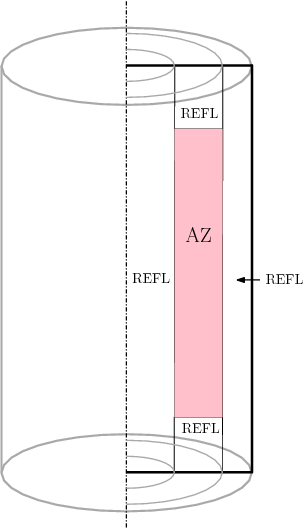
\includegraphics[scale=.4]{images/Hermes/VHTR.png}
\end{frame}

\begin{frame}[t]
  \frametitle{Example calculation}
  \vspace*{-.3cm}
  \centering\textcolor{structure.bg!95!blue}{ Group fluxes distribution }\\[3em]
    \hspace*{-.6cm}
  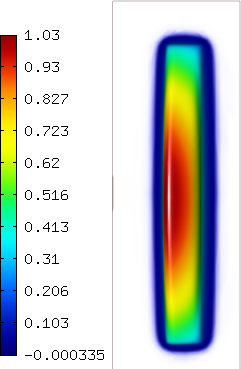
\includegraphics[height=4.5cm]{images/Hermes/hp1/screen001.png}~
  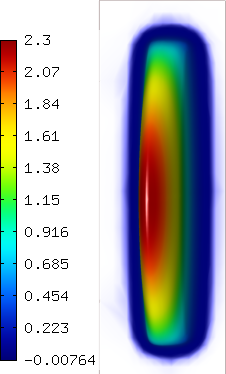
\includegraphics[height=4.5cm]{images/Hermes/hp1/screen002.png}~
  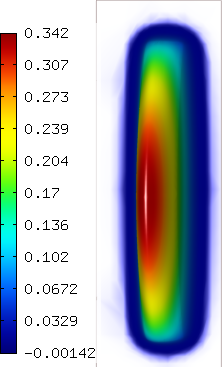
\includegraphics[height=4.5cm]{images/Hermes/hp1/screen003.png}~
  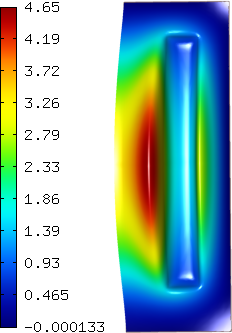
\includegraphics[height=4.5cm]{images/Hermes/hp1/screen004.png}
\end{frame}

%\begin{frame}[t]
%  \frametitle{Example calculation}
%  \vspace*{-.3cm}
%  \centering\textcolor{structure.bg!95!blue}{ Adaptive $h$-refinement }\\[3em]
%    \hspace*{-.6cm}
%  \includegraphics[height=4.75cm]{images/Hermes/href/screen001-transparent.png}\hspace*{-.3cm}
%  \includegraphics[height=4.75cm]{images/Hermes/href/screen002-transparent.png}\hspace*{-.3cm}
%  \includegraphics[height=4.75cm]{images/Hermes/href/screen003-transparent.png}\hspace*{-.3cm}
%  \includegraphics[height=4.75cm]{images/Hermes/href/screen004-transparent.png}
%\end{frame}

%\begin{frame}[t]
%  \frametitle{Example calculation}
%  \vspace*{-.3cm}
%  \centering\textcolor{structure.bg!95!blue}{ Adaptive $h$-refinement }\\[.35em]
%  \only<1>{
%    \hspace*{.75cm}
%    \includegraphics[height=6.75cm]{images/Hermes/href/conv_dof-transparent.png}
%  }
%  \only<2>{
%    \hspace*{.75cm}
%    \includegraphics[height=6.75cm]{images/Hermes/href/conv_cpu-transparent.png}
%  }
%\end{frame}

\begin{frame}[t]
  \frametitle{Example calculation}
  \vspace*{-.3cm}
  \centering\textcolor{structure.bg!95!blue}{ Adaptive $hp$-refinements }\\[3em]
  \only<1>{  
  \hspace*{-.6cm}
  \includegraphics[height=4.75cm]{images/Hermes/hp1/screen005-transparent.png}\hspace*{-.3cm}
  \includegraphics[height=4.75cm]{images/Hermes/hp1/screen006-transparent.png}\hspace*{-.3cm}
  \includegraphics[height=4.75cm]{images/Hermes/hp1/screen007-transparent.png}\hspace*{-.3cm}
  \includegraphics[height=4.75cm]{images/Hermes/hp1/screen008-transparent.png}
  }
%  \only<2>{
%  \hspace*{-.6cm}  
%  \includegraphics[height=4.75cm]{images/Hermes/hp2/screen005-transparent.png}\hspace*{-.3cm}
%  \includegraphics[height=4.75cm]{images/Hermes/hp2/screen006-transparent.png}\hspace*{-.3cm}
%  \includegraphics[height=4.75cm]{images/Hermes/hp2/screen007-transparent.png}\hspace*{-.3cm}
%  \includegraphics[height=4.75cm]{images/Hermes/hp2/screen008-transparent.png}\\[.5cm]
%  \begin{center} Progressively changing power iteration tolerance during adaptation \end{center}
%  }
\end{frame}

\begin{frame}[t]
  \frametitle{Example calculation}
  \vspace*{-.3cm}
  \centering\textcolor{structure.bg!95!blue}{ Adaptive $hp$-refinement }\\[.35em]
  \only<1>{
    \hspace*{.75cm}
    \includegraphics[height=6.75cm]{images/Hermes/hp1/conv_dof-transparent.pdf}
  }
  \only<2>{
    \hspace*{.75cm}
    \includegraphics[height=6.75cm]{images/Hermes/hp1/conv_cpu-transparent.pdf}
  }
%  \only<3>{
%    \hspace*{.75cm}
%    \includegraphics[height=6.75cm]{images/Hermes/hp1/conv_cpu-transparent.png}
%  }
%  \only<4>{
%    \hspace*{.75cm}
%    \includegraphics[height=6.75cm]{images/Hermes/hp2/conv_cpu-transparent.png}
%  }
 \end{frame}
  


\section{Some connections}
\begin{frame}[c]
	\frametitle{Nodal method \& adaptive FEM ?}
	\begin{itemize}
	    \item Various kinds of error estimation techniques (Ainsworth \& Oden)
	        \begin{itemize}
	            \item \emph{Hierarchic error indicators}
	        \end{itemize}
	\end{itemize}
	
	\begin{tikzpicture}
			\node[mybox, inner ysep=1.2ex, inner xsep=0ex] (Model) {%
				\begin{minipage}{1.03\textwidth}\centering
					\small
          \begin{itemize}
            \item	Find $\flfl \in \VV:\quad \A(\flfl,\vv) = \L(\vv),\quad \forall \vv\in \VV$
            \item Let $\VV$ represent a low order FE space (e.g. $p = 1$)
          \end{itemize}
				\end{minipage}
			};
		\node[fancytitle] (Modelt) at (Model.north) {\small Original problem};

  \uncover<2->{
			\node[mybox, below=.5cm of Model.south, anchor=north, inner ysep=1.2ex, inner xsep=0ex] (Method) {%
				\begin{minipage}{1.03\textwidth}\centering
					\small
					\begin{itemize}
            \item Let $\overline\VV = \VV \oplus \EE$
            \item Looking for the solution $\overline\flfl = \flfl + \mathbf{e}$ in 
                  the higher order FE space $\overline\VV$
            \item $\mathbf{e}$ ... component of $\overline\flfl$ lying in $\EE$
                \begin{itemize}
                    \item if the \emph{saturation assumption} holds, provides a good
                  approximation to the true error for $\flfl\in \VV$
                \end{itemize}
          \end{itemize}
				\end{minipage}
			};
		\node[fancytitle] (Methodt) at (Method.north) {\small Hierarchic space decomposition};
				}
	\end{tikzpicture}    

	
		\vspace{.15cm}\color{Black}\hrule width 5.1cm
		\begin{thebibliography}{\textwidth} 
			\beamertemplatearticlebibitems
			\bibitem[EST]{EST}
			\footnotesize{M. Ainsworth and J. T. Oden},
			\newblock \scriptsize{A-posteriori error estimation in finite element analysis}
			\newblock {\scriptsize \color{white!80!black}John Wiley \& Sons, Inc., 2000}
		\end{thebibliography}		
	
\end{frame}
    %!!!!!!!!!!! RENAME
\begin{frame}[t]
	\frametitle{Iterative methods}            
	\begin{itemize}
	    \item Close connection to error estimation (e.g. Bank)
	\end{itemize}
	\vspace{-.5em}
	\begin{center}
		    \begin{tikzpicture}
            \node[mybox, inner ysep=0pt] (boxx) {%
                \begin{minipage}[t]{.7\textwidth}\centering
                    $$
                    \begin{aligned}
                        \dkr[<2>]{\A(\flfl^{(n+\frac12)},\vv)} = \L(\vv) - \dkg[<3>]{\A(\mathbf{e}^{(n)},\vv)},\quad \vv\in\VV \\
                        \dkb[<4>]{\A(\mathbf{e}^{(n+1)},\mathbf{w}) = \L(\mathbf{w}) - \A(\flfl^{(n+\frac12)},\mathbf{w}),\quad \mathbf{w}\in\EE}
                    \end{aligned}
                    $$\\[.1em]
                \end{minipage}
            };
            \node[fancytitle] (boxxt) at (boxx.north) {\small Iterative form};
            \end{tikzpicture}
    \end{center}
	\vspace{-.5em}    
	    \begin{itemize}
	        \item Close connection to the nodal method: $\dkr[<2>]{\MM\flfl} = \QQ - \dkg[<3>]{\DD\flfl}$.
	        \uncover<4->{\item\dkb{Solution for the nodal expansion coefficients and correction factors}}
	    \end{itemize}   
	\uncover<5->{    
    \begin{center}\alert{We believe that results of the iteration analysis for this method
    could improve our theoretical understanding of the nodal method.}\end{center}}
	\vspace{.15cm}\color{Black}\hrule width 5.1cm
		\begin{thebibliography}{\textwidth} 
			\beamertemplatearticlebibitems
			\bibitem[ES2T]{ES2T}
			\footnotesize{R. E. Bank},
			\newblock \scriptsize{Hierarchical Bases and the Finite Element Method}
			\newblock {\scriptsize Acta Numerica (1997)}
		\end{thebibliography}
\end{frame}


\section{Conclusion}
\begin{frame}[c]
	\frametitle{Conclusion and final thoughts}
	 \begin{itemize}
	 	\item CMFD accelerated nodal method is a highly efficient 
	 	      solution technique for systems of (not only, but mostly) elliptic PDEs on structured meshes\pause
	 	\item It is lacking behind the adaptive FEM in terms of
	 	\begin{itemize}
	 	    \item flexibility
	 	    \item detailed spatial resolution
	 	    \item theoretical background\pause
	 	\end{itemize}
	 	\item The ideas behind it naturally appear in some FEM-dominated areas too
	 	\begin{itemize}
	 		\item methods using hierarchical bases
	 		\item domain decomposition with coarse mesh acceleration\pause
	 	\end{itemize}
	 	\item We should be able to bring the two methods even closer to each other by considering the
	 	      DG approximation on the FEM side
	 \end{itemize}
\end{frame}

\begin{frame}[c]
	\frametitle{}
	\begin{center}
	  \LARGE\emph{ Thanks for attention }\\[.5em]
	  \hrule width \textwidth\vspace{.5em}
	  \normalsize\color{structure} mhanus@kma.zcu.cz
	\end{center}
\end{frame}



\end{document}
